\subsection{Datamodel}
Het Datamodel bestaat uit 4 \textbf{objecten} wat in zijn geheel leid naar de uitendelijke data die naar de frontend wordt gestuurd.
Deze objecten zijn Item Definition, Item Value, Visual Component en ItemVisual.

\whitespace[2]
\textbf{Item value}: De item value is de entiteit dat de data/content encapsuleert van het systeem.
Om de data structuur zo flexibel mogelijk te houden is er gekozen om de item value 1 of meerdere referenties naar andere item values te geven.
Dit is gedaan zodat de item value structuur een geneste strucuuur wordt en gemakkelijk door de interface gerenderd kan worden.
De daat werkelijke data/content is opgeslagen in de fields van de item value.
Deze fields maken gebruik van een abstacte base class die er voor zorgt dat er meerde data types in een item value gebruikt kunnen worden.
De lijst van huidige field values is String,Bool,Int en api.
Doordat de gebruik is gemaakt is van een abstractie, kunnen er acties uitgevoerd worden op de fields.
Een speciale van deze fields is het api field, dit field heeft de mogelijkheid om dynamisch content op te halen.
Dit wordt nu gebruikt bij het ophalen van up to date data op te halen van youtube of andere video platformen. 

\whitespace[2]
\begin{graphic}
    \captionsetup{type=figure}
    \caption{klassen diagram ItemValue}
    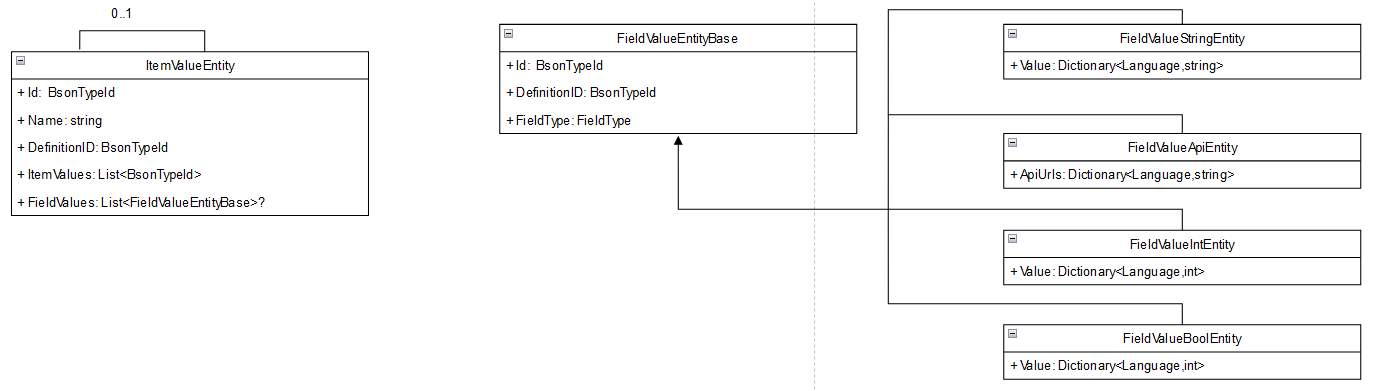
\includegraphics[scale=0.7]{ItemValueEntityClassDiagram.png}
    \label{fig:ItemValueEntityClassDiagram}
\end{graphic}

\whitespace[2]
\textbf{Item Definition}: Om structuur te geven aan de Item values wordt er gebruik gemaakt van een item Definition.
        De belangrijkste functionaliteit van de definition is om aan te geven welke velden er op verschillende items zitten en welke daarvan verplicht zijn.

\whitespace[2]
\begin{graphic}
    \captionsetup{type=figure}
    \caption{klassen diagram ItemDefinition}
    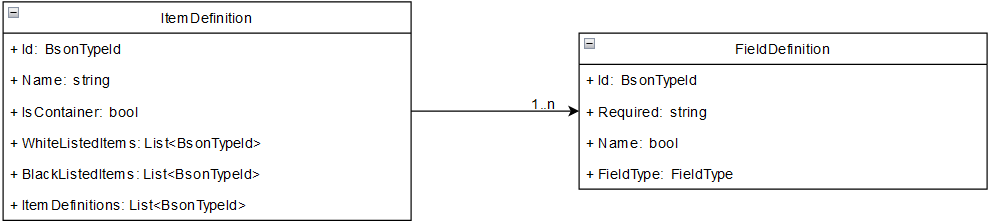
\includegraphics[scale=0.8]{ItemDefinitionClassDiagram.png}
    \label{fig:ItemDefinitionClassDiagram}
\end{graphic}

\whitespace[2]
\textbf{VisualComponent}: Om de data te renderen moeten er components gebruikt worden in de frontend om dit af te handelen waar nodig.
De VisualComponent wordt gebruikt om deze componenten aan te geven welke er zijn en welke definition er bij hoordt.

\whitespace[2]
\begin{graphic}
    \captionsetup{type=figure}
    \caption{Klassen diagram VisualComponent}
    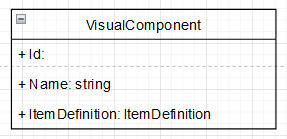
\includegraphics[scale=0.8]{VisualComponentEntityClassDiagram.png}
    \label{fig:VisualComponentEntityClassDiagram}
\end{graphic}

\whitespace[2]
\textbf{ItemVisual}: Dit is het object dat de VisualComponent en de Item Value samen voegt tot een geheel waardoor er content gerenderd kan worden op de pagina.
Verder geeft dit object ook aan welke mogelijke stijling of layout op het item moet worden toegepast.

\whitespace[2]
\begin{graphic}
	\captionsetup{type=figure}
	\caption{Klassen diagram ItemVisual}
	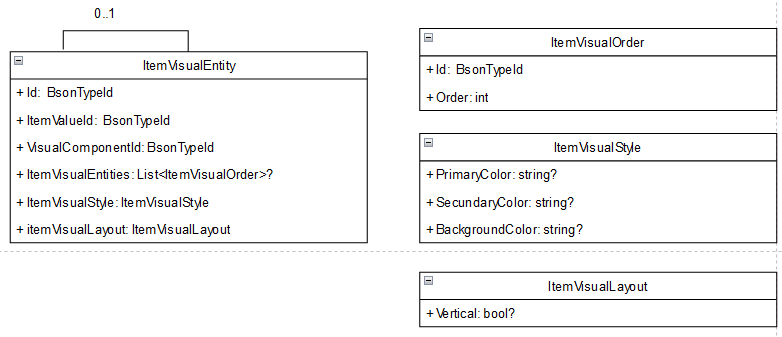
\includegraphics[scale=0.8]{ItemVisualEntityClassDiagram.png}
	\label{fig:ItemVisualEntityClassDiagram}
\end{graphic}

\whitespace[2]
Om de data te renderen op een froentend wordt de itemVisual geparesed naar een ItemVisualDTO zie figuur \ref{fig:ItemVisualDTOClassDiagram}.

\whitespace[2]
\begin{graphic}
	\captionsetup{type=figure}
	\caption{Klassen diagram ItemVisual}
	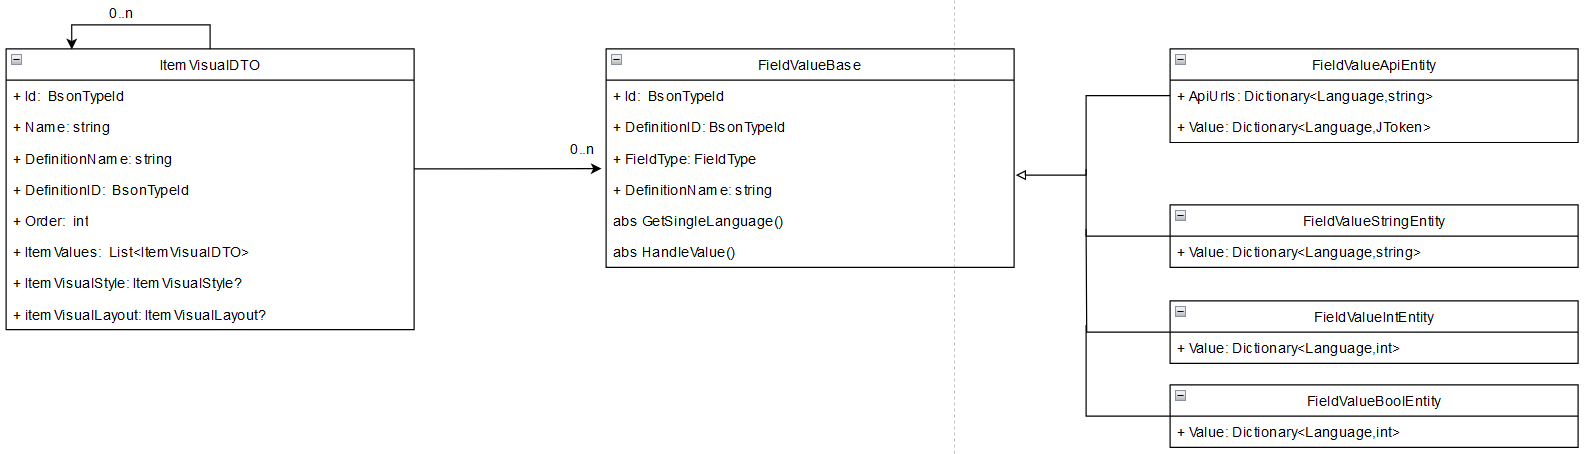
\includegraphics[scale=0.7]{ItemVisualDTO.png}
	\label{fig:ItemVisualDTOClassDiagram}

\end{graphic}
